\clearpage
%//==============================--@--==============================//%
\subsection[2.4 Limitadores e Fixadores]{\hspace*{0.075 em}\raisebox{0.2 em}{$\pmb{\drsh}$} Limitadores e Fixadores}
\label{subsec:limitadores-e-fixadores}

%//==============================--@--==============================//%
\subsubsection[2.4.1 Limitadores]{$\pmb{\rightarrow}$ Limitadores}

\begin{quote}
    ``O \textbf{limitador} (\textit{clipper}) é um circuito cuja tensão de saída tem um limite superior, um limite inferior, ou ambos os limites, sendo proporcional à tensão de entrada enquanto estes limites não são atingidos.''\cite{medeiros:ICEE}
\end{quote}

\vspace{-1.5em}
\begin{figure}[H]
    \centering
    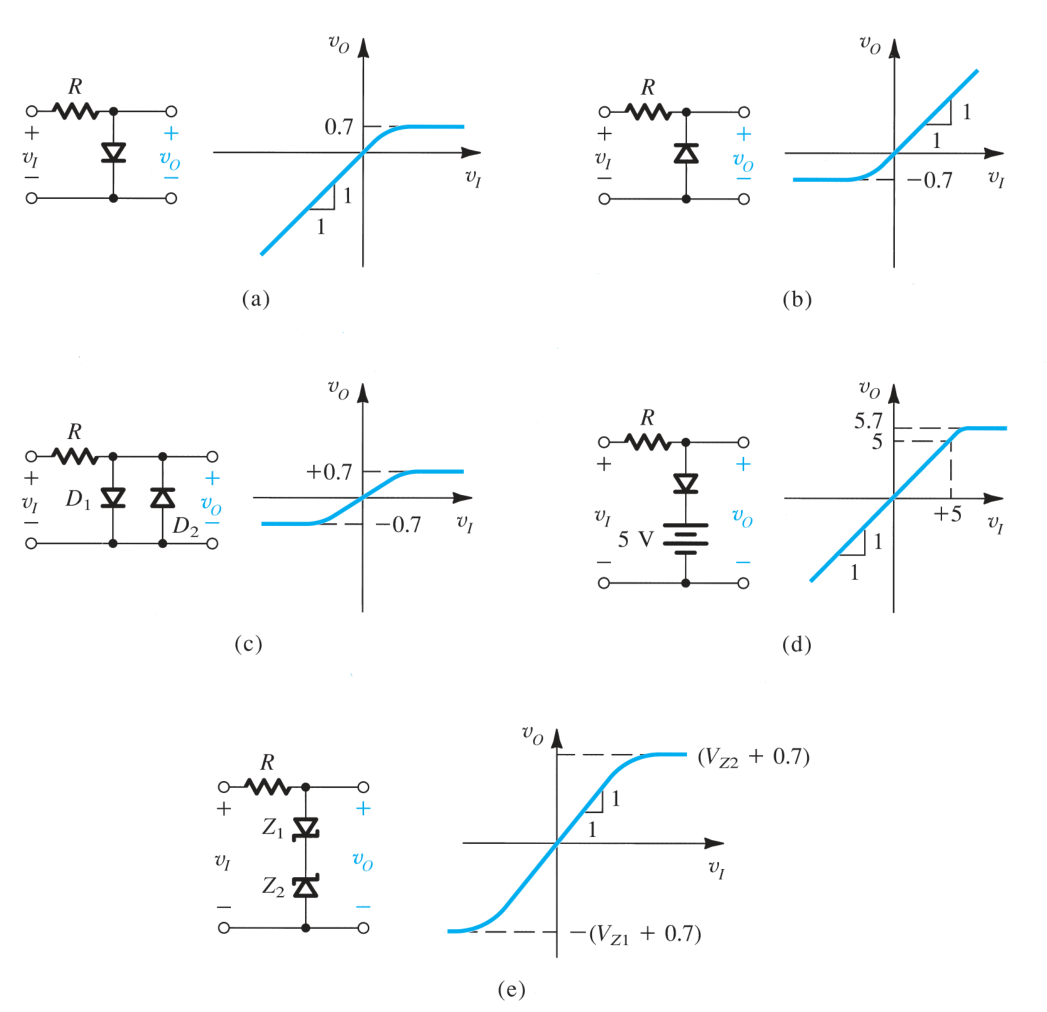
\includegraphics[width=0.8\linewidth]{img/2/limitadores.png}
    \caption{``A variety of basic limiting circuits.''\cite{sedra-smith:microelectronic-circuits}}
    \label{fig:limitadores}
\end{figure}

%//==============================--@--==============================//%
\subsubsection[2.4.2 Fixadores]{$\pmb{\rightarrow}$ Fixadores}

\begin{quote}
    ``O \textbf{fixador} (\textit{clamper}) é um circuito cuja tensão de saída tem a mesma forma que a tensão de entrada, mas em que o seu valor minimo, ou o seu valor máximo, é fixo e independente da tensão de entrada.''\cite{medeiros:ICEE}
\end{quote}

\vspace{-1.5em}
\begin{figure}[H]
    \centering
    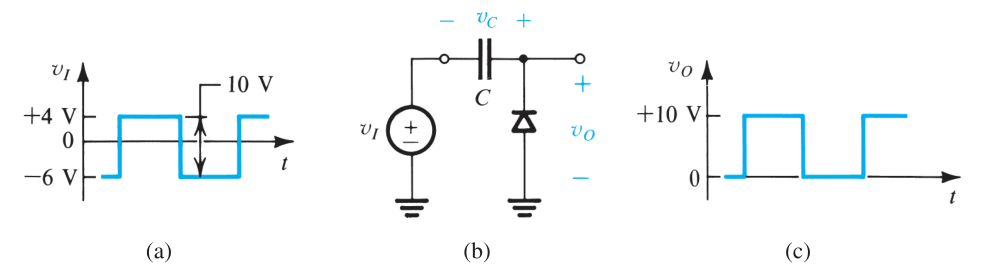
\includegraphics[width=0.85\linewidth]{img/2/fixador.png}
    \caption{``The \textbf{clamped capacitor} or \textbf{dc restorer} with a square-wave input and no load. Because of the polarity in which the diode is connected, the capacitor will charge to a voltage $v_C$ with the polarity indicated and equal to the magnitude of the most negative peak of the input signal. Subsequently, the diode turns off and the capacitor retains its voltage indefinitely.''\cite{sedra-smith:microelectronic-circuits}}
    \label{fig:fixador}
\end{figure}
%//==============================--@--==============================//%